% Chapter Template
\chapter{The LHC and the CMS Experiment} \label{Chapter2} 


\section{Introduction}
This thesis' chapter outlines the main characteristics of the Large
Hadron Collider (LHC) and of the Compact Muon Solenoid (CMS)
detector. 
``An accelerator propels charged particles, such as protons or electrons, at high speeds, close to the speed of light. They are then smashed either onto a target or against other particles circulating in the opposite direction. By studying these collisions, physicists are able to probe the world of the infinitely small.

When the particles are sufficiently energetic, a phenomenon that
defies the imagination happens: the energy of the collision is
transformed into matter in the form of new particles, the most massive
of which existed in the early Universe. This phenomenon is described
by Einstein’s famous equation E=mc2, according to which matter is a
concentrated form of energy, and the two are interchangeable.

The Large Hadron Collider is the most powerful accelerator in the world. It boosts particles, such as protons, which form all the matter we know. Accelerated to a speed close to that of light, they collide with other protons. These collisions produce massive particles, such as the Higgs boson or the top quark. By measuring their properties, scientists increase our understanding of matter and of the origins of the Universe. These massive particles only last in the blink of an eye, and cannot be observed directly. Almost immediately they transform (or decay) into lighter particles, which in turn also decay. The particles emerging from the successive links in this decay chain are identified in the layers of the detector.''

%----------------------------------------------------------------------------------------
%	SECTION 1
%----------------------------------------------------------------------------------------
\section{The Large Hadron Collider}

The LHC~\cite{Brning2004LHCDR} is a circular particle accelerator
located at the CERN laboratories in Geneva operating since 10
September 2008. It is
designed to accelerate hadrons (like protons, Lead-ions, Xenon-ions) and to
operate at the centre-of-mass energy of 14\TeV.
The circular ring is installed in a tunnel of a 27 kilometers where
the Large Electron Positron collider~\cite{Lep:designReport} was
previously located.\\
A graphic rapresentation of CERN accelerator
complex is shown in Figure~\ref{fig:cern} where the particle
accelerations begins at the LINAC, foregoing booster, PS and SPS, in
order. The LHC consists of accelerating components as well as
supercondicting magnets to focus the hadrons, keep them on the right
trajectory and squeeze them tight together right before the
collision point. 

\begin{figure}[h]
\centering
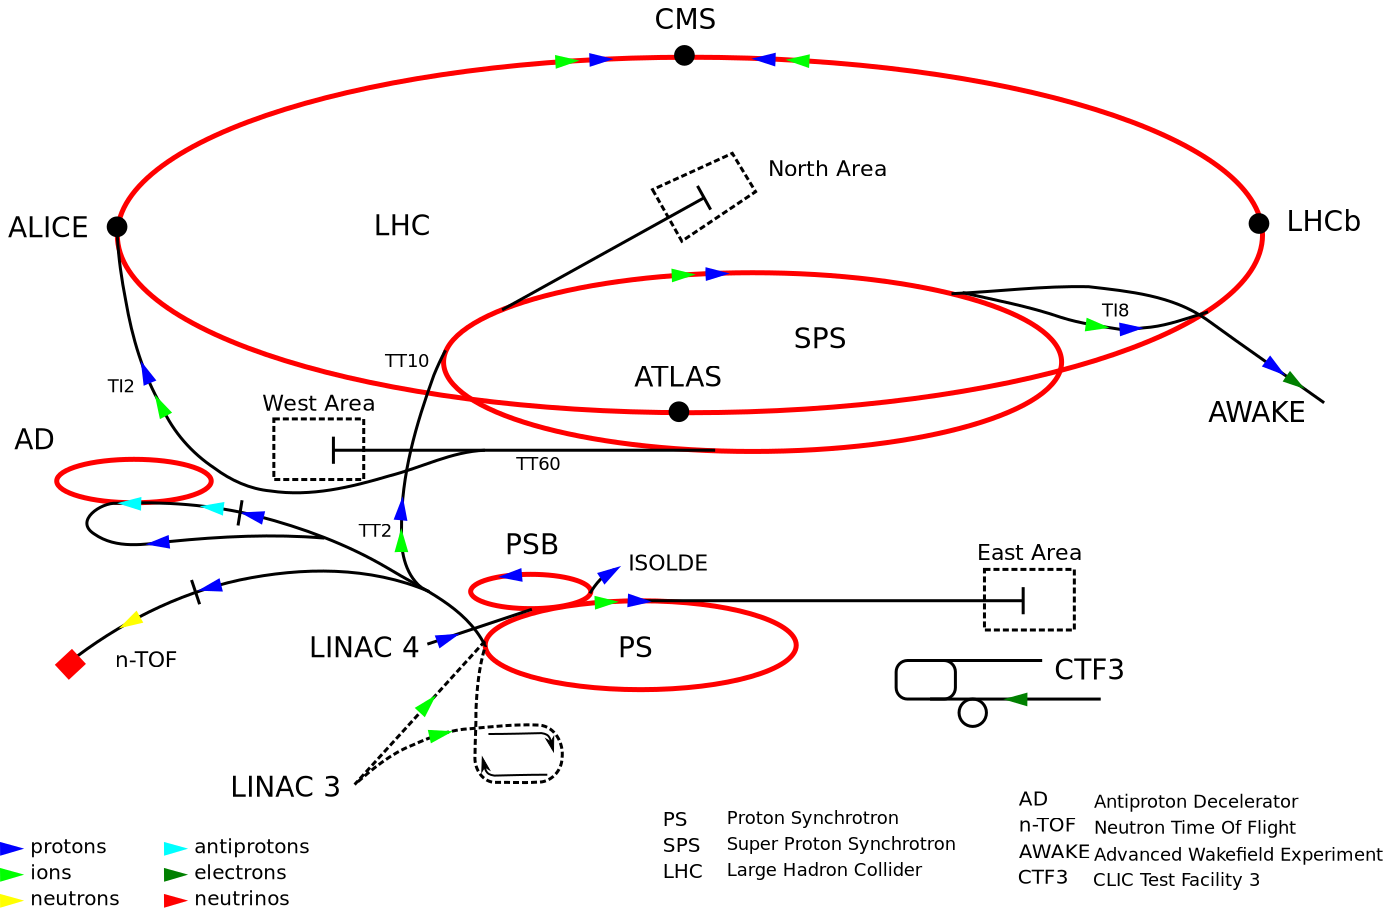
\includegraphics[width=0.75\textwidth]{Figures/c2/Cern-accelerator-complex.png}
\vspace*{3mm}
\caption{The LHC is the largest ring (top) in a complex chain of particle accelerators. The smaller machines are used in a chain to help boost the particles to their final energies and provide beams to a whole set of smaller experiments, which also aim to uncover the mysteries of the Universe~\cite{Mobs:2197559}}
\label{fig:cern}
\end{figure}

The protons are accelerated in opposite directions in two distinct
accelerator tubes which cross at four interactions points where the
protons are made to collide. At each of the interaction points along the ring,
four experiments are located with the aim to reconstruct the
sub-atomic particles which are made at the moment of a high energy
collision. The protons are grouped in bunches which are
accelerated in steps using the full accelerator chain consisting in a linear
accelerator, boosters, syncrotons and, at the end, they are injected
into the LHC with an energy of 540\GeV where a system of
superconducting magnets futher accelerate them up to 13\TeV. Every
25 ns collisions between proton bunches occour meaning 40 million
bunch crossing per second. At full regime during data taking time
period about 2800 bunches travel in the LHC rings and each bunch is
made of up to $1.1\times10^{11}$ protons.

The four experiments located at the four interaction points are
ALICE~\cite{alice_2008} (A Large Ion Collider Experiment),
ATLAS~\cite{atlas_2008} (A Toroidal LHC ApparatuS),
CMS~\cite{cms_2008} and LHCb~\cite{lhcb_2008} (Large Hadron Collider
beauty), refer to Figure~\ref{fig:cern}. ALICE experiment is designed
to study the presence and the properties of the hypotetical
quark-gloun plasma formed during heavy ions collisions, LHCb is
designed to be very sentitive in analysing the properties of the B
mesons. The last two, ATLAS and CMS are general purpose detectors
designed to investigate a vast range of physics scenarios starting
from the search and discovery of the Higgs boson to extra dimensions
and dark matter. \\

The accelerator-dependent features and parameters which are important for a
physics analysis are the instantaneous and integrated luminosity, the
number, in the same bunch crossing, of simultaneous collisions and the
center-of-mass energy of the proton-proton collisions.

The instantaneous luminosity is defined as a time dipendent
parameter, $d\mathcal{L}/dt$, which correlates the number of collisions
($N$) in a certain amount of time ($t$) and the cross section of a
given process through the relation:
\begin{equation}
\label{eq:instalumi}
\frac{dN}{dt} \: = \: \frac{d\mathcal{L}}{dt}\sigma
\end{equation}

The unit of the instantaneous luminosity is $b^{-1}s^{-1}$, where 1
barn $= 10^{-24} \ cm^2$ and it depends on the number of bunches in
the proton beam, on the number of protons per bunch and on the beam
optics. \\
The integrated luminosity is the integral of the instantaneous
luminosity over time, and relates the cross section of a
given process to the number of events $N$ of that process:
\begin{equation}
\label{eq:intelumi}
\mathcal{L} \:=\: \int \frac{d\mathcal{L}}{dt} dt \: = \: \frac{N}{\sigma}
\end{equation}


\begin{figure}[h]
  \noindent
  \makebox[\textwidth]{
  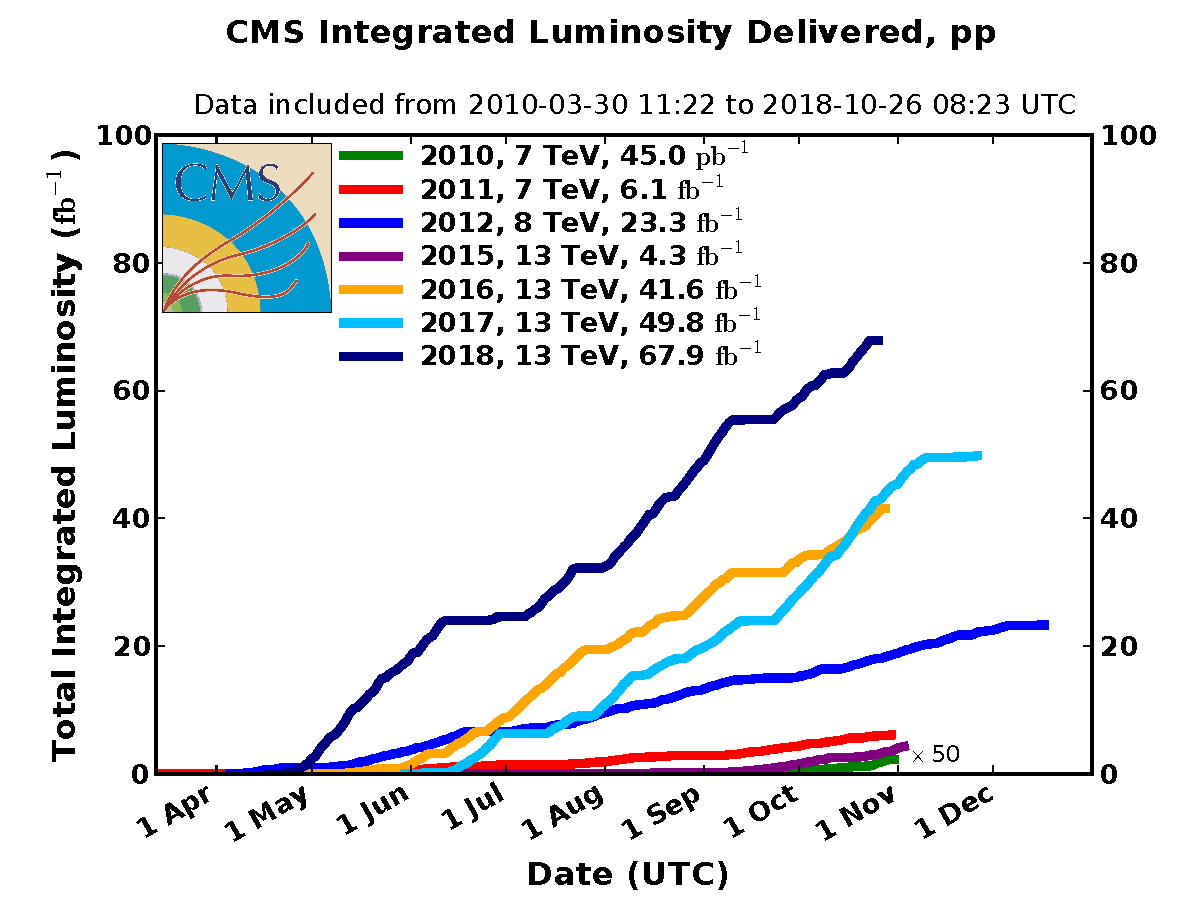
\includegraphics[width=.50\textwidth]{Figures/c2/int_lumi_cumulative_pp_2.pdf}
  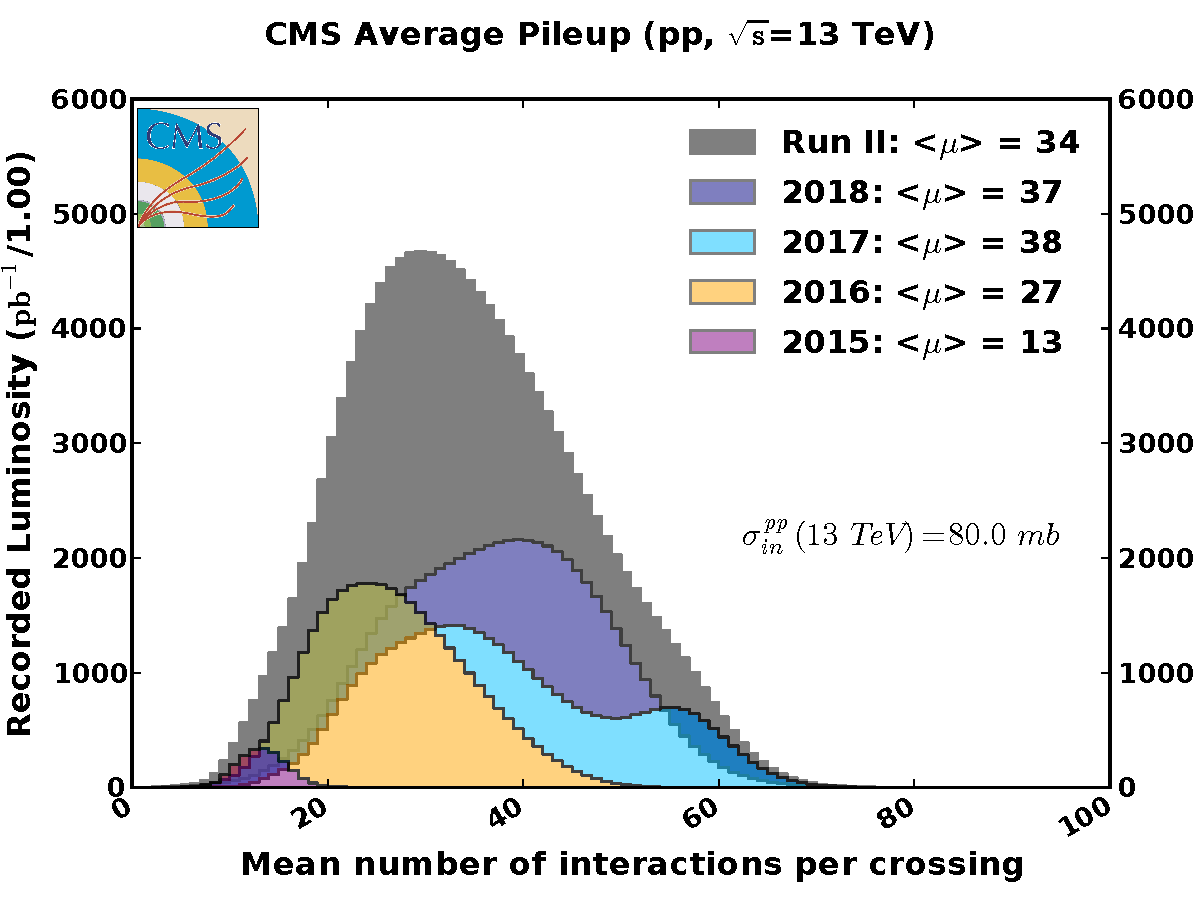
\includegraphics[width=.50\textwidth]{Figures/c2/pileup_allYears_run2.pdf}}\\
  \makebox[\textwidth]{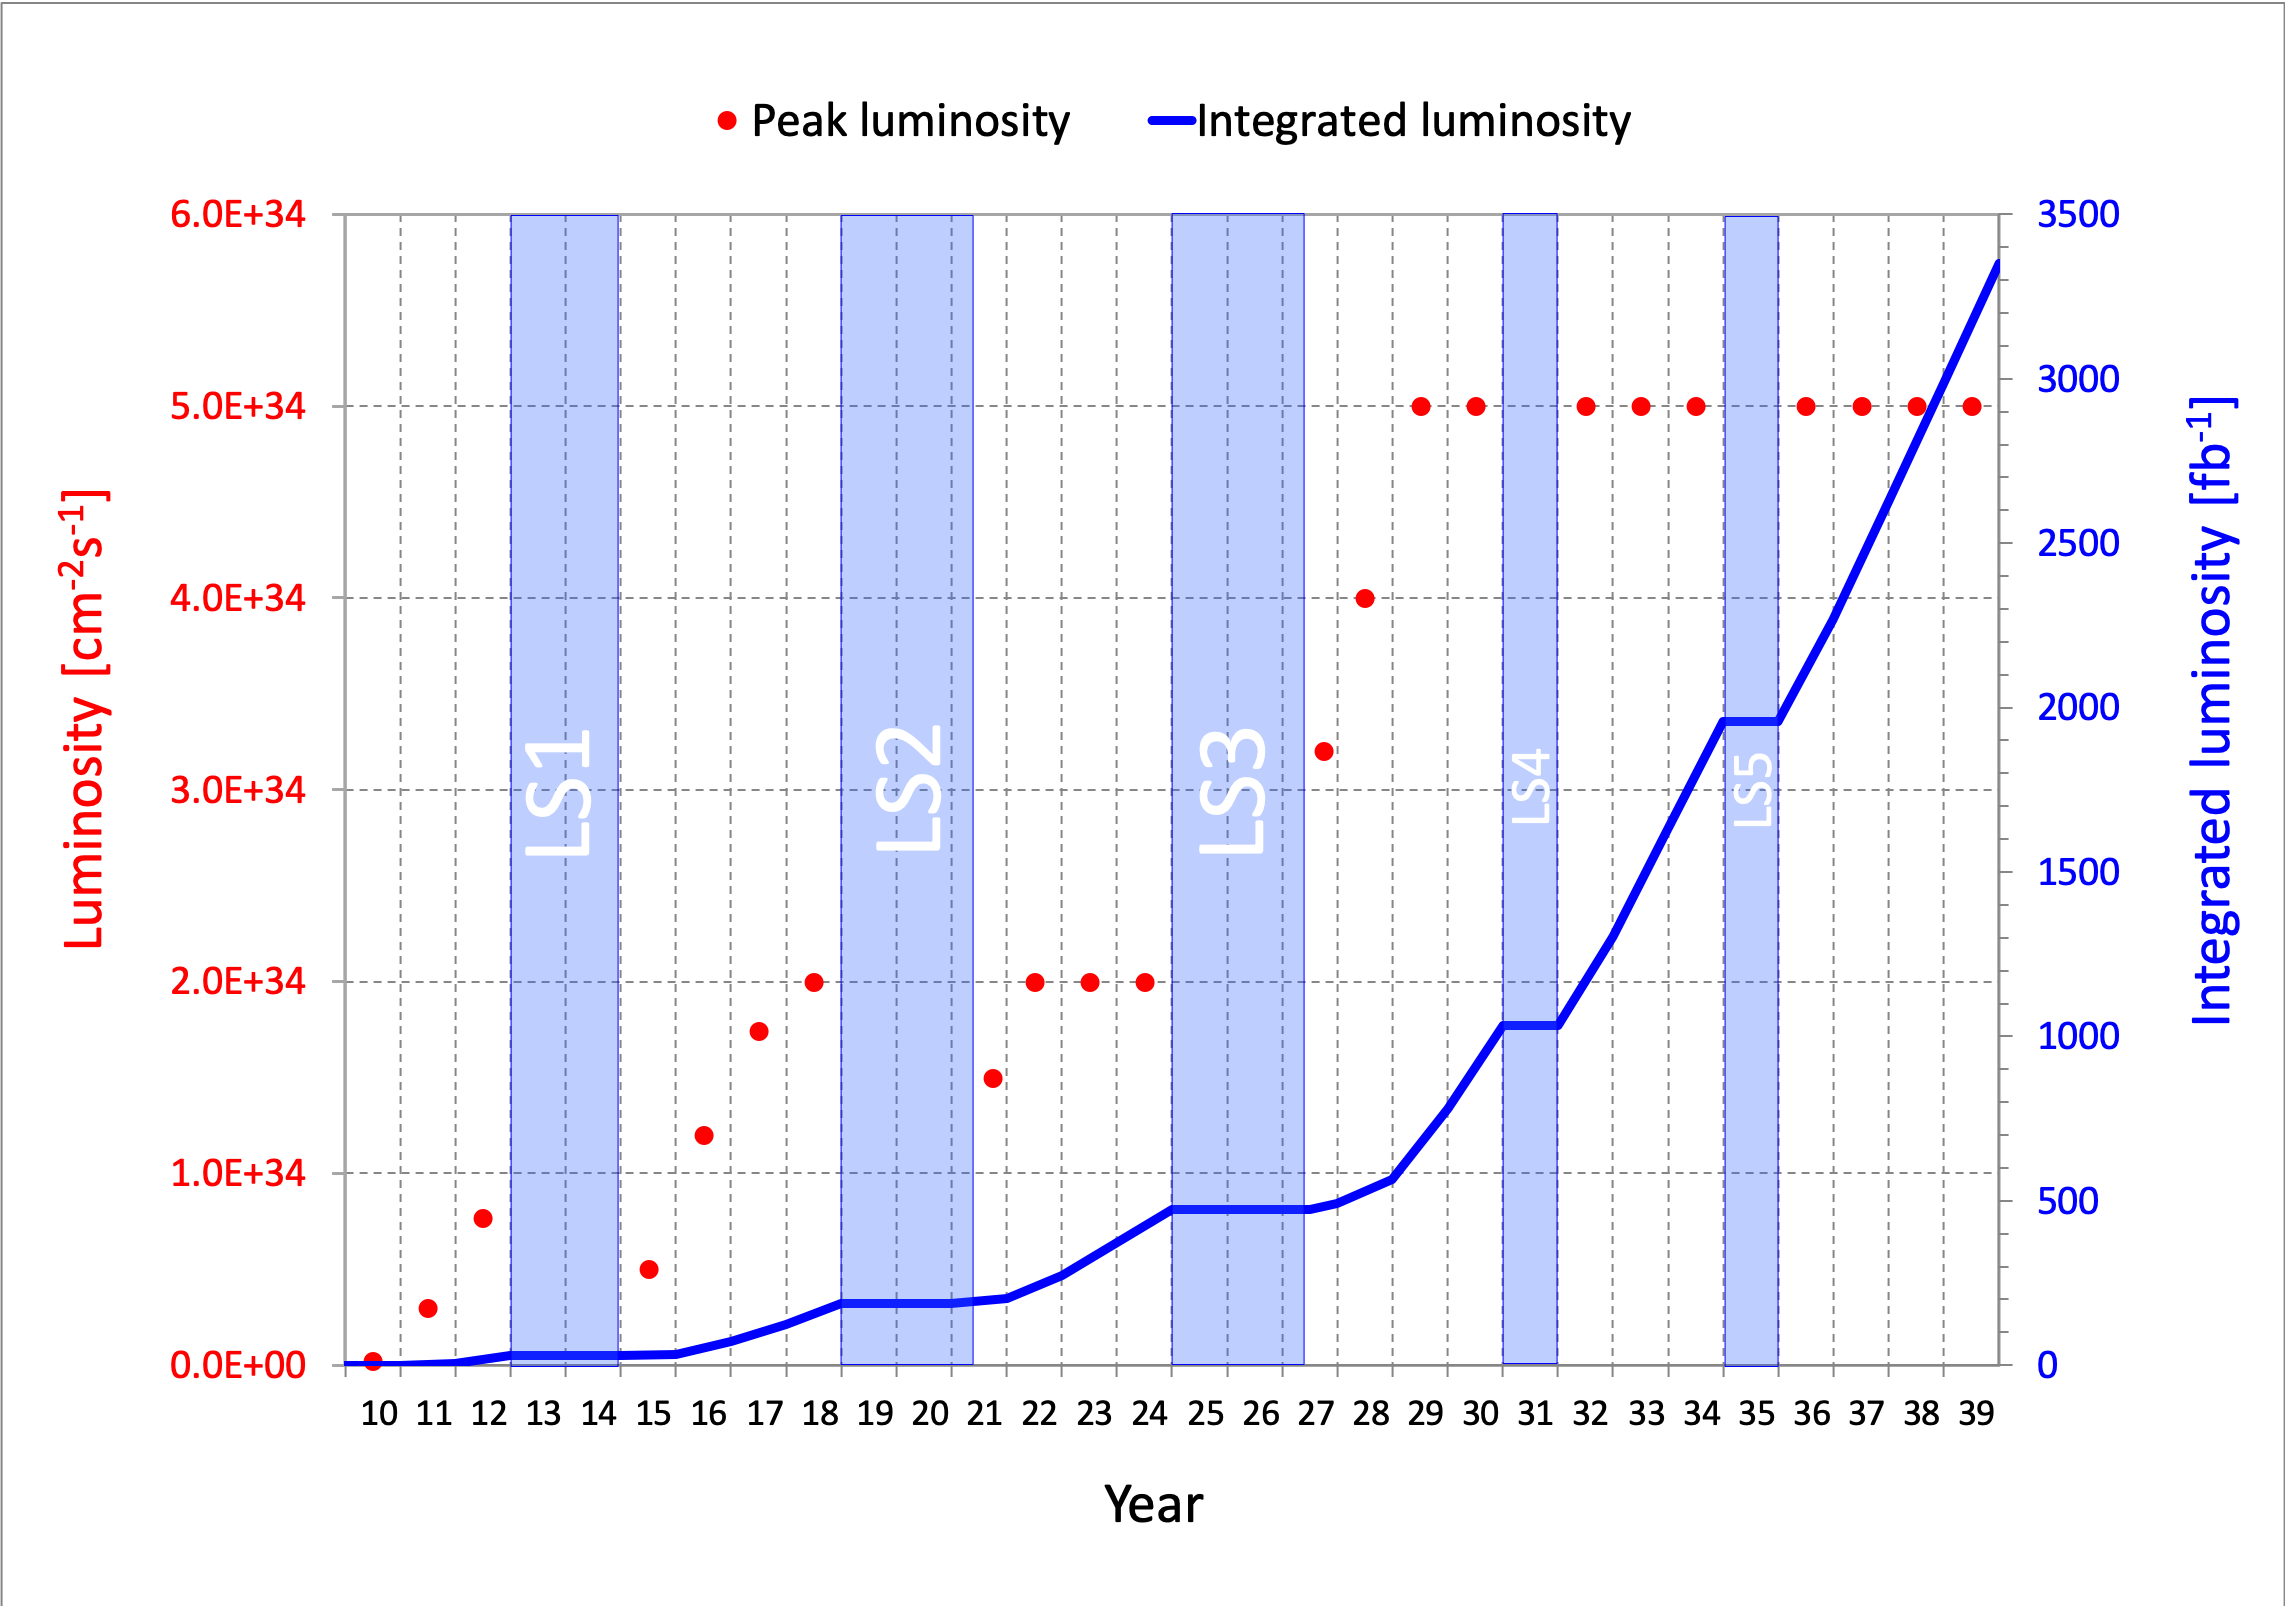
\includegraphics[clip,trim=0.2cm 0.2cm 0.2cm 0.2cm, width=.60\textwidth]{Figures/c2/Lumi.png}}
  \caption{Top-left: integrated luminosity collected by the CMS
    experiment; top-right: distribution of the average number of
    interactions per crossing (pileup) for pp collisions in 2015
    (purple), 2016 (yellow), 2017 (azzure), 2018 (periwinkle), and
    full Run2 (gray),~\cite{webpage_lumi}. Bottom: scheduled and
    projected integrated and instantaneous luminosity at the LHC~\cite{webpage_lhc}.}
  \label{fig:lumi}
\end{figure}

The LHC was designed to deliver an instantaneous luminosity
of $10^{34}cm^{-2}s^{-1}$. Figure~\ref{fig:lumi} (top-left and central
plots) shows the schedule of the Large Hadron Collider from the start
to the following years of operations. The LHC has delivered two
outstanding runs of data taking: the first phase, Run1 (2010-2012) at
center-of-mass energy of 7 and 8\TeV and total delivered integrated
luminosity of $29.4\ fb^{-1}$; the first 3 years of data taking proved
the physics potentiality of the LHC with, among others, the Higgs boson
discovery. The secon run, Run2 (2015-2018) started after 2 years Long
Shutdown when the machine and the detectors were confirmed and
consolidate to be able to run at the full capacity with 
center-of-mass energy of 13\TeV and total delivered integrated
luminosity of $162.9\ fb^{-1}$.\\
The increase in luminosity over the
years was the result of improvements in the beam quality and optics which
led to an higher number of pp collisions per bunch crossing. This
quantity is refered as pileup, PU which is shown in the top-right plot
in Figure~\ref{fig:lumi}. The average <PU> for Run2 is 34, this larger
number of collision per bunch crossing on one hand
expands the physics reach of the CMS and ATLAS experiments because of
the higher probability of an episode of a rare collision, on the
other hand most of the PU interactions pollute the information of the
event because they are moslty soft and less interesting to look for
new physics models posing the detector in the place to be able to
disantangle and reconstruct each single pp collision. 

\section{The Compact Muon Solenoid}


\begin{figure}[h]
\centering
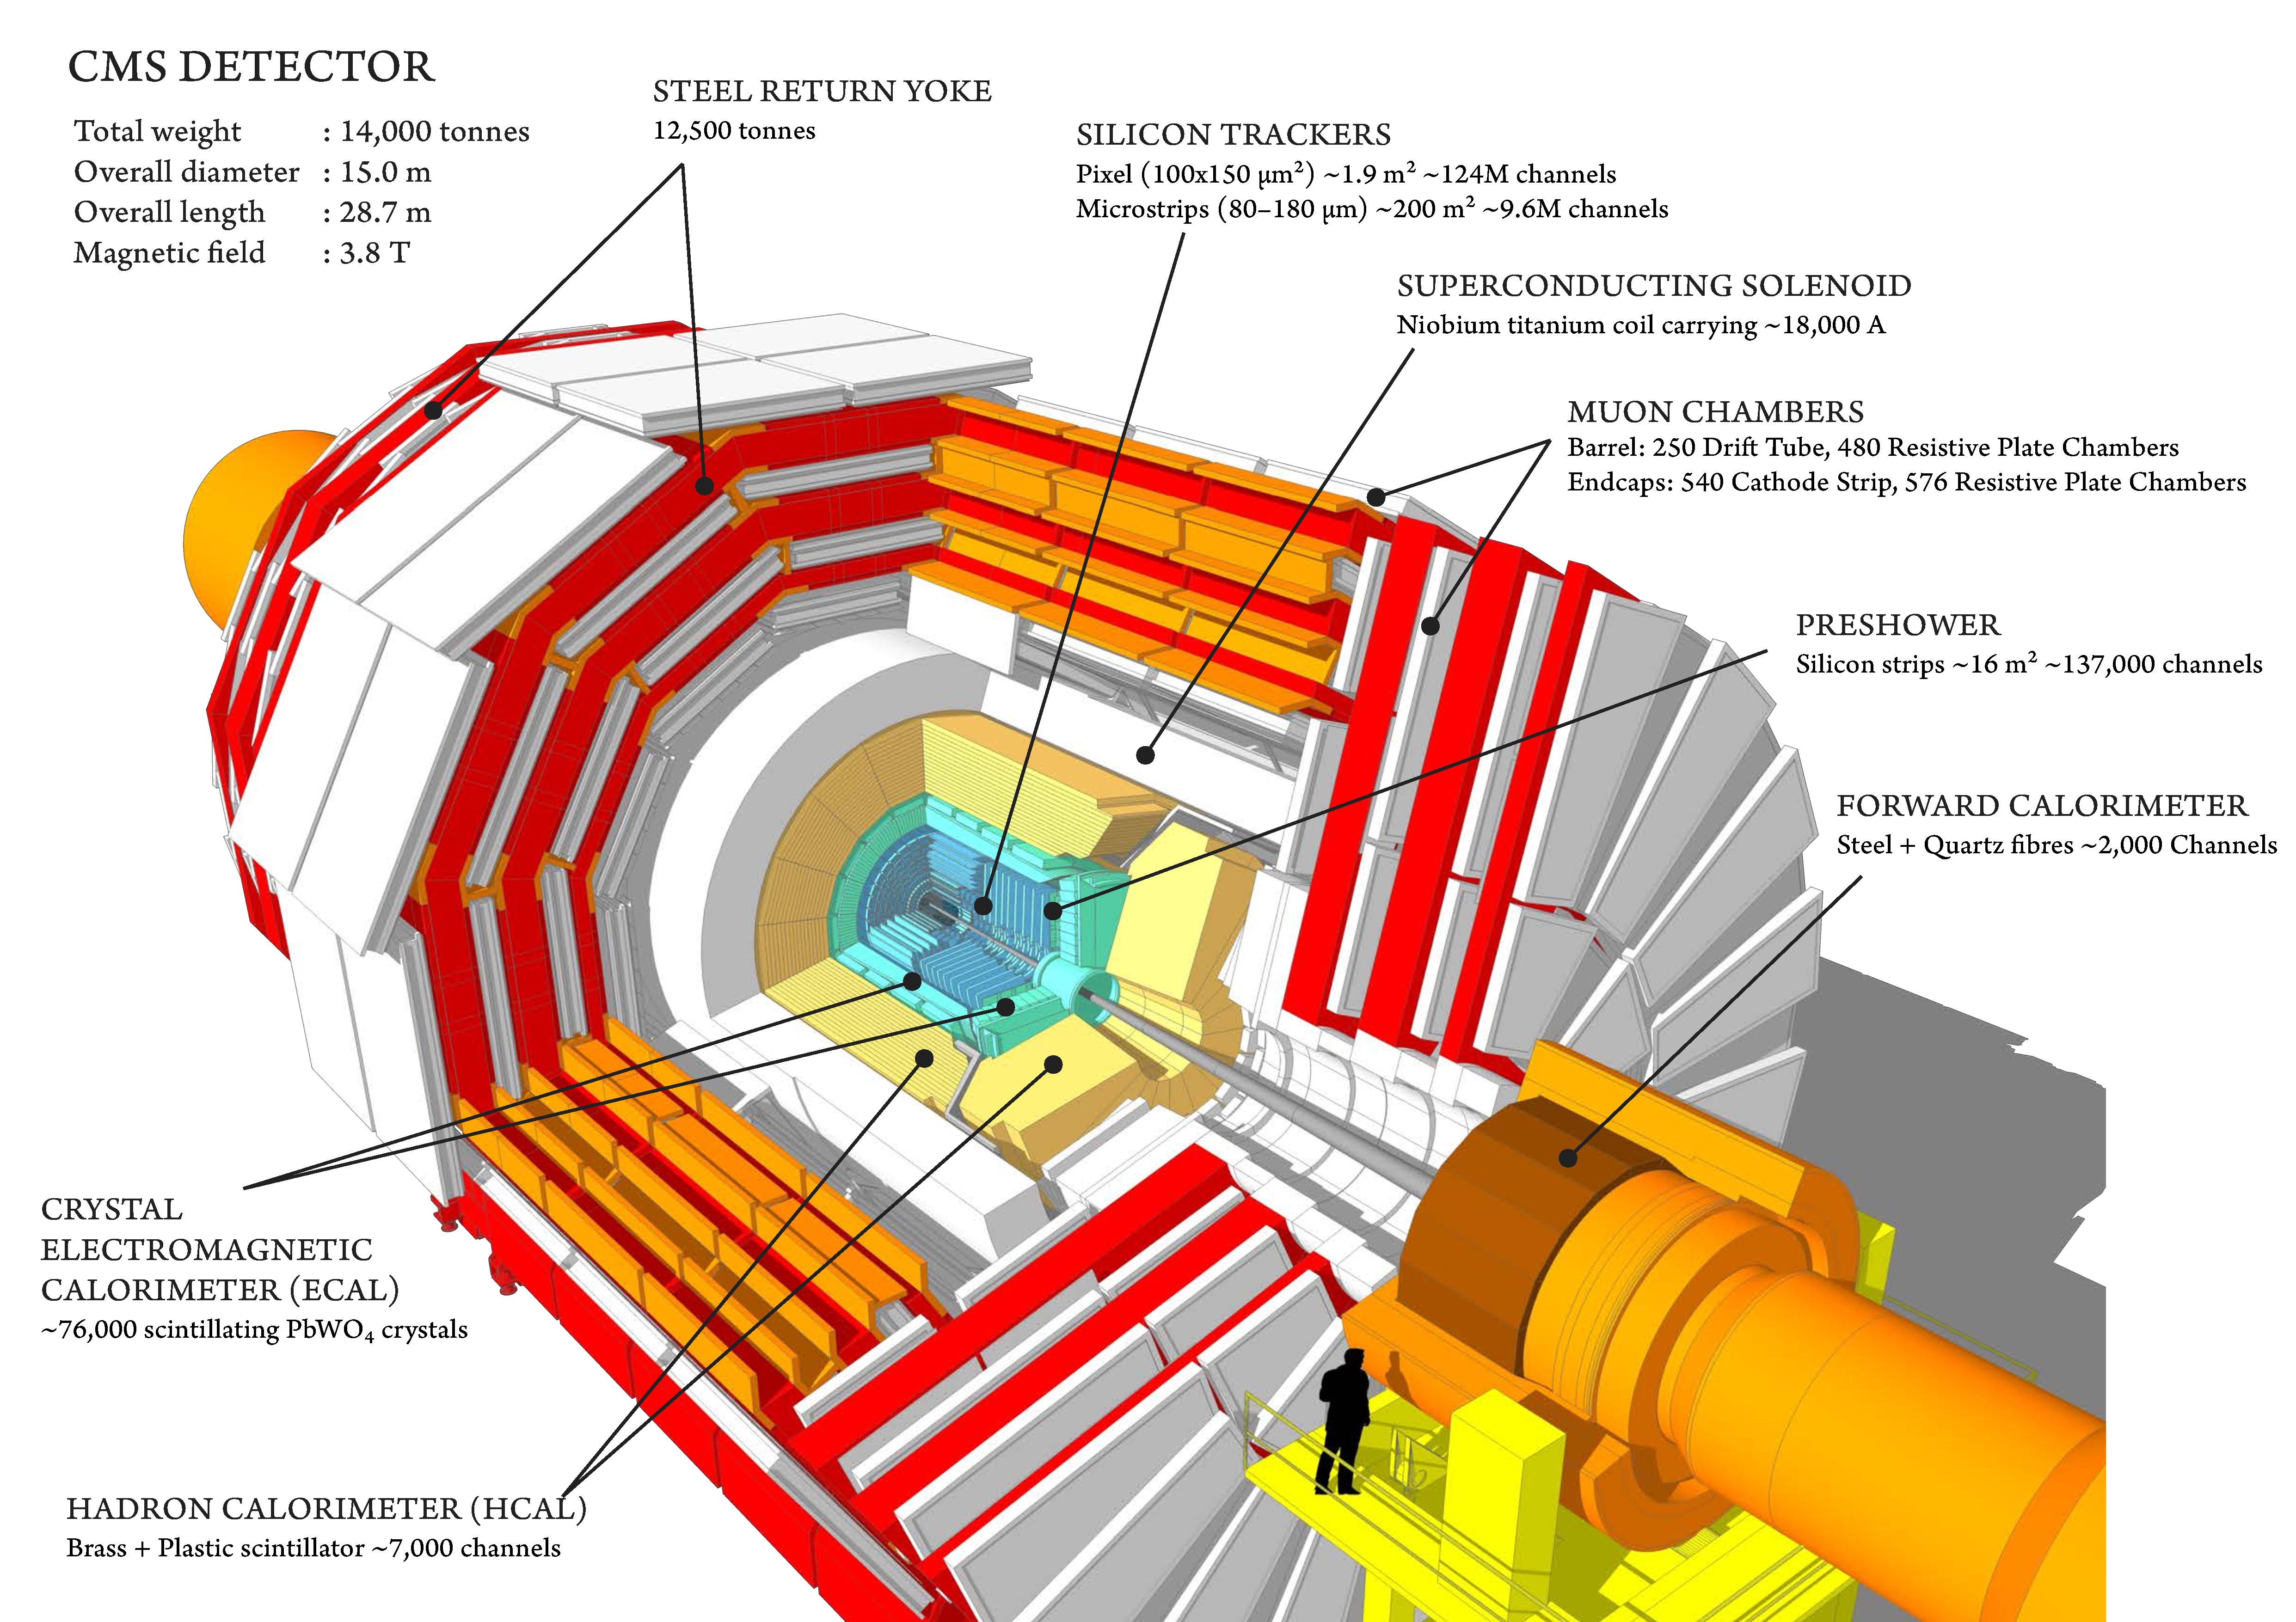
\includegraphics[width=0.75\textwidth]{Figures/c2/cms_160312_06-compressed.pdf}
\vspace*{3mm}
\caption{A scheme of the CMS detector and its parts~\cite{webpage_cms}.}
\label{fig:cern}
\end{figure}
 
\clearpage
\subsection{The Large Hadron Collider}
\subsection{Experiments at the LHC}
\subsection{Design and performance of the LHC}

%-----------------------------------
%	SECTION 2
%-----------------------------------
\section{The CMS experiment}
\subsection{The CMS coordinate system} 
\subsection{The solenoid magnet} 
\subsection{The charged-particle tracker} 
\subsection{The electromagnetic calorimeter} 
\subsection{The hadronic calorimeter} 
\subsection{The muon detector} 
\subsection{Triggering and data acquisition} 
\section{Event reconstruction}\label{sec:reconstruction}
\subsection{Track reconstruction} 
Electron reconstruction is based on the combination of tracker and
ECAL information in a Gaussian Sum Filter (GSF)
track~\cite{Khachatryan:2015hwa}, which accounts for possible
bremsstrahlung from the electron.
Electrons are reconstructed within the geometrical acceptance of the
CMS tracking system, $|\eta|<2.5$.
Identification criteria based on the electromagnetic shower shape, track
quality, track impact parameters with respect to the primary vertex,
and isolation are used to select signal electrons and reduce the rate
of mis-identified and background electrons (referred to as ``fake
electrons'' hereafter).

Muons are reconstructed by combining the information of the tracker
and of the muon
spectrometer~\cite{Sirunyan:2018fpa}.
The geometric compatibility between these separate measurements is
used in the further selection of muons. Muons are required to have
$\abseta<2.4$ to fall inside the geometric acceptance of the muon
detector.
All muons considered for analysis must pass the loose working point as
specified by the MUO POG, in addition to a number
of other loose criteria on isolation and their impact parameters with
respect to the PV.
It is also possible to require muons to be synchronized with the bunch
crossing that has triggered, using the time measurements provided by
the muon sub-detectors, the RPCs (``RPC time'' or $t_{\mathrm{RPC}}$)
and the combined measurements of the DTs and CSCs (``combined time''
or $t_{\mathrm{comb}}$)~\cite{muon_oot}.
In particular, $t_{\mathrm{RPC}}$ ($t_{\mathrm{comb}}$) is only used
if it is measured with more than 1 (7) degrees of freedom.
If $t_{\mathrm{RPC}}$ and $t_{\mathrm{comb}}$ are both available,
they must lie within $-10\ns$ and $+10\ns$.
If only $t_{\mathrm{comb}}$ is available, then it must be within
$-45\ns$ and $+20\ns$.
If $t_{\mathrm{comb}}$ is unavailable, no timing requirement is
applied.

\subsection{Reconstruction performances}
\clearpage
